\documentclass{article} % article doctype, possible font size range from 8pt to 20pt with not all being avaiable.
\title{\huge Willy The Robot Movement Research}
\author{Jeroen van 't Hul\\S1139163  \and Thomas Zwaanswijk\\s1089273 \and Tom van den Noort\\s1101124}
\date{\parbox{\linewidth}{\centering%
	\today\endgraf\bigskip
	Supervisor \hspace*{3cm} Main Stakeholder \endgraf\medskip
	Mischa Mol \hspace*{3cm} Ilja Clabbers \endgraf\bigskip
	Windesheim Zwolle\endgraf}} 


% include packages
\usepackage{graphicx}
\usepackage{caption}
\usepackage{mathabx}
\usepackage{wrapfig}
\usepackage[margin=1.0in]{geometry} % sets page margin, 2.0in is default.
\usepackage{titlesec}
\usepackage{hyperref}
\usepackage[table,xcdraw]{xcolor}
\usepackage{float}
\usepackage[export]{adjustbox}
\usepackage{todonotes}
\usepackage{indentfirst}
\usepackage{blindtext}
\usepackage{scrextend}
%\usepackage{siunitx}
%\usepackage{multirow}	% used for table multirow support
%\usepackage{longtable} % Allows tables to roll over into a new page.
\usepackage[nottoc,numbib]{tocbibind} % Adds bibliography / references to TOC and numbers that section.
\usepackage{array}
\usepackage{footnote}

% ----- custom commands ----- %
% Wrapper for paragraph command. Forces newline after paragraph title
\newcommand{\myparagraph}[1]{\paragraph{#1}\mbox{}\\} % Without \mbox{} all newlines will be ignored, making the first sentence appear on the same line as a paragraph title.
% monospace codeblock
\def\code#1{\texttt{#1}}
% changing the ToC depth in the document enviroment
\newcommand{\changelocaltocdepth}[1]{%
	\addtocontents{toc}{\protect\setcounter{tocdepth}{#1}}%
	\setcounter{tocdepth}{#1}%
}

\newcolumntype{L}[1]{>{\raggedright\let\newline\\\arraybackslash\hspace{0pt}}m{#1}}
\newcolumntype{C}[1]{>{\centering\let\newline\\\arraybackslash\hspace{0pt}}m{#1}}
\newcolumntype{R}[1]{>{\raggedleft\let\newline\\\arraybackslash\hspace{0pt}}m{#1}}

\makesavenoteenv{tabular}
\makesavenoteenv{table}

\setcounter{tocdepth}{2} % only part,chapters,sections, subsections appear in ToC

\addtokomafont{labelinglabel}{\sffamily}

\DeclareCaptionFormat{cancaption}{#1#2#3\par} % Normal format actually
\DeclareCaptionLabelFormat{cancaptionlabel}{#1}
\captionsetup[figure][number]{format=cancaption,labelformat=cancaptionlabel}
\graphicspath { {images/}{../images/} }

\begin{document}
\maketitle

\begin{figure}[H]
\centering
\includegraphics[width=12 cm]{WTRLogo.png}
\end{figure}
\thispagestyle{empty}
\newpage
\setcounter{page}{1}
\tableofcontents
\newpage

% Sections
\section{Introduction}
This research is meant to create an inventory of the current state of the movements WTR\ref{trm::WTR} is capable of performing.
In addition, this document contains a list of proposed improvements in order to increase the accuracy of the autonomous driving.
By creating a list of the range of movement WTR can perform and noting any defects or issues with those, it should become easier to create a proper list of improvements.
Several sections will deal with the sensors, how they benefit the robot and their mounting as well.
\newpage

\section{Current State}
In its current state, WTR is capable of autonomous movement, but if the previous group is to be believed, the current driving capabilities are reminiscent of "a drunken Pole".
This is obviously undesirable, since WTR is meant to be a way of drawing in potential students with an interest in robotics and programming at Windesheim, or those with an interest in engineering.
Having WTR be a danger to the people around it, the walls, cupboards or any other obstacles would be more likely to scare scare away potential students than get them to study at Windesheim.

\subsection{Controlled Movement}
Before getting WTR to drive autonomously, it should be moved to a safe location using the attached Dualshock PS3 controller \cite{dualshock}.
While the \href{https://windesheim-willy.github.io/WillyWiki/components/joystick.html}{wiki} will claim that WTR can be controlled by holding the select button on the PS3 dualshock controller and moving the right joystick, that is incorrect.
The left joystick is used to move the robot, assuming the controller is held with the joysticks at the bottom of the controller.
Having to hold select means that the robot should essentially have a "dead-man's switch" [\ref{trm::dms}].
Unfortunately, in the current state releasing select while having the joystick held in any direction causes WTR to continually repeat said movement, so if it is turning and the controller is accidentally dropped it will continue to turn in the direction it was heading.
This is obviously a dangerous oversight, and should be corrected ASAP [\ref{trm::ASAP}].

\subsection{Autonomous Movement}
The autonomous driving is fairly advanced.
While there are some more technicalities, the core system can be divided into two aspects, navigation/localization planning and the execution of the planned instructions.

\subsubsection{Localization/Navigation}
There was some confusion early on about the use of April tags, but after a meeting with the previous groups it turned out that those are only used for calibration and to use as convenient targets for WTR to drive to.
As such, these can be largely ignored if a solution is found for WTR to keep track of its location in another manner, such as an IMU or a sufficiently accurate GPS sensor.

The current autonomous movement suffers from a lack of feedback.
In the "Brain" node, it is assumed that every instruction is executed mostly without issue, while in reality, the pivoting rear wheels and the friction from the wheel rubbing against the frame cause some serious discrepancy.

The navigation uses a map of the area based on data from the LIDAR.
There are some issues with creating a new map, but those are being looked into.
By manually driving WTR while running a specially made program, it can store where obstacles are located.
This map can then be manually edited to seal off certain areas where WTR should not be moving, such as between tables where it would barely fit.
After this, WTR can be calibrated to start in a certain position, and then be set to drive autonomously to a chosen goal in the predesignated area.

One note that should be considered is that the local planner has been changed from what might be stated in other documentation.
As of 28/02/2019, the planner used has been changed from \code{base\_ local\_ planner} to \code{teb\_ local \_ planner}, which offers more options when it comes to robot shapes, sizes and methods of steering.
These approximate WTR's situation more closely, and as such the change has been made.
In the current iteration, WTR can drive relatively smoothly, although it does still experience some small issues in terms of movement speed, which the \code{teb} planner judges on the lower side, so it at times lacks the power to move forward.

\subsubsection{Executing Instructions}
Another issue with the autonomous driving is that the ROS move\_ base uses default recovery/emergency behaviours [\ref{trm::recpat}].
These are based on robots which can move in a different manner from WTR.
Most of them assume that the robot can rotate along a center axis which is located in the exact center of the robot, meaning that when it turns in a circle, no parts stick out in any direction more than the default state.
WTR turns around on an axis located in between the two front wheels, meaning the rear sticks out further than expected, causing unwanted collisions.

The ultrasonic sensors are not used at the moment, if the previous group is to be believed.
This is an area of clear improvement, as they can be used to prevent collisions and detect humans at a close range.

Another factor that was revealed was that the odometry data is being spoofed to some degree to correct for any drifting in reference points.
This is a major issue, since that would be mean that the longer WTR is driving around without rebooting/recalibrating, the worse the performance would become.
Since at the time of writing this document WTR cannot drive forward in a straight line without entering recovery behaviour movement patterns, this means that eventually it would become stuck in a permanent loop of that behaviour.

\newpage

\section{Closed Loop Drive Control}
\subsection{Introduction}
WTR currently has an "open loop control system" \cite{openloop} that controls how it turns and drives.
There are no sensors used to provide feedback, which could be used to control and adjust accordingly.
This is a major drawback, because the robot is already quite difficult to control; While it does not move very quickly, the motors have a lot of power behind them.
Should one of the wheels receive less power from the motor than the other, it will affect the trajectory of WTR, resulting in poor path-finding.

\subsection{System Description}
\label{subs::SysDes}
WTR consists of two powered wheels at the front and two wheels on pivot each at the rear.
The two powered wheels each have a separate electrical motor.
This set-up is quite sensitive to small variations between the two motors, though it does allow for a good range of movements.

\subsection{Current Setup}
An Arduino Mega 2560 (based on the ATmega2560 \cite{ardMega} is used to receive input from the laptop used as core control unit, and then translates that into instructions for the motors from the mobility scooter.
The commands sent are translated into a corresponding power output of the wheels via the integrated motor controller of the scooter.
Two commands can be sent, one for the speed of the motors and one for rotation.
Both commands fall within a range of 100 to -100.
Unfortunately, this set-up does not allow for independent control of both motors, but an appropriate model of the system could be used to approximate that level of control.

\subsection{Improvements}
Two sensors will be added to the axles of both wheels, which allow WTR to use the speed and rotation of the wheels as feedback.
These sensors will be controlled via a micro-controller, likely a Arduino Uno \cite{ardUno}, since those are already available and simple to use.
This set-up would allow for an integrated closed loop control system using negative feedback.
An overview can be found in figure~\ref{fig::cllp}.
\begin{figure}[H]
\centering
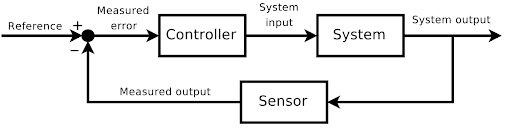
\includegraphics[width=12 cm]{controlmodel.png}
\caption{Example of the closed loop control system}
\label{fig::cllp}
\end{figure}
\newpage

\subsection{Model Of Control}
\subsubsection{Base}
As explained in 'System Description' \ref{subs::SysDes}, the motors can only be controlled through two output variables.
These two variables are \code{drive} output and \code{turn} output, both limited to values between 100 and -100.
Originally, these input were sent directly from the Arduino Mega, which applied the limits to the received values.
An overview can be found in table~\ref{tab::varoverview}
\begin{figure}[H]
\begin{tabular}{|l|l|c|c|l|l|}
\hline
\textbf{Nr.} & \textbf{Variable(s)} & \textbf{Left(+)} & \textbf{Right(-)} & \textbf{Min} & \textbf{Max} \\ \hline
1 & Input Turn 	& \multicolumn{2}{c|}{Turn\_ Input} 				& - 		& -		\\ \hline
2 & Input Drive 	& \multicolumn{2}{c|}{Drive\_ Input} 				& - 		& - 		\\ \hline
3 & Drive Output & \multicolumn{2}{c|}{Drive\_ Output = Drive\_ Input}	& -100 	& +100 	\\ \hline
4 & Turn Output 	& \multicolumn{2}{c|}{Turn\_ Output = Turn\_ Input}	& -100	& +100	\\ \hline
\end{tabular}
\caption{Overview of inputs and outputs of the original system}
\label{tab::varoverview}
\end{figure}

\subsubsection{Control Model}
To be able to create a controller which can control the speed of the wheels depending on input based on both the drive and input values, a direction definition has to be set up first.
The definition is:
\begin{itemize}
\item \code{Turning left will be a positive input value and a corresponding positive left wheel speed and a negative or lesser right wheel speed. Turning right will correspond with a negative input value and a positive right wheel speed and a negative or lesser left wheel speed}
\item \code{Moving forward corresponds with a positive input value and wheel speed, while moving backwards corresponds with a negative input value and negative wheel speed}
\end{itemize}
This is illustrated in figure \ref{fig::controldiagram}.
This system allows for a calculation of a separated reference speed per wheel, which is shown in table \ref{tab::closedoverview}, row 4.
The total reference speed can be calculated as shown in table \ref{tab::closedoverview}, row 5.
The offset per wheel (labelled as \code{Error}) can be calculated by subtracting the measured speed from the reference speed, as shown in table \ref{tab::closedoverview}, row 7.
As the speed of the wheels cannot be individually controlled, both errors have to be combined into the drive output and turn output variables.
Additionally, a controller $(C_m(S))$ has to be integrated.

\begin{figure}[H]
\centering
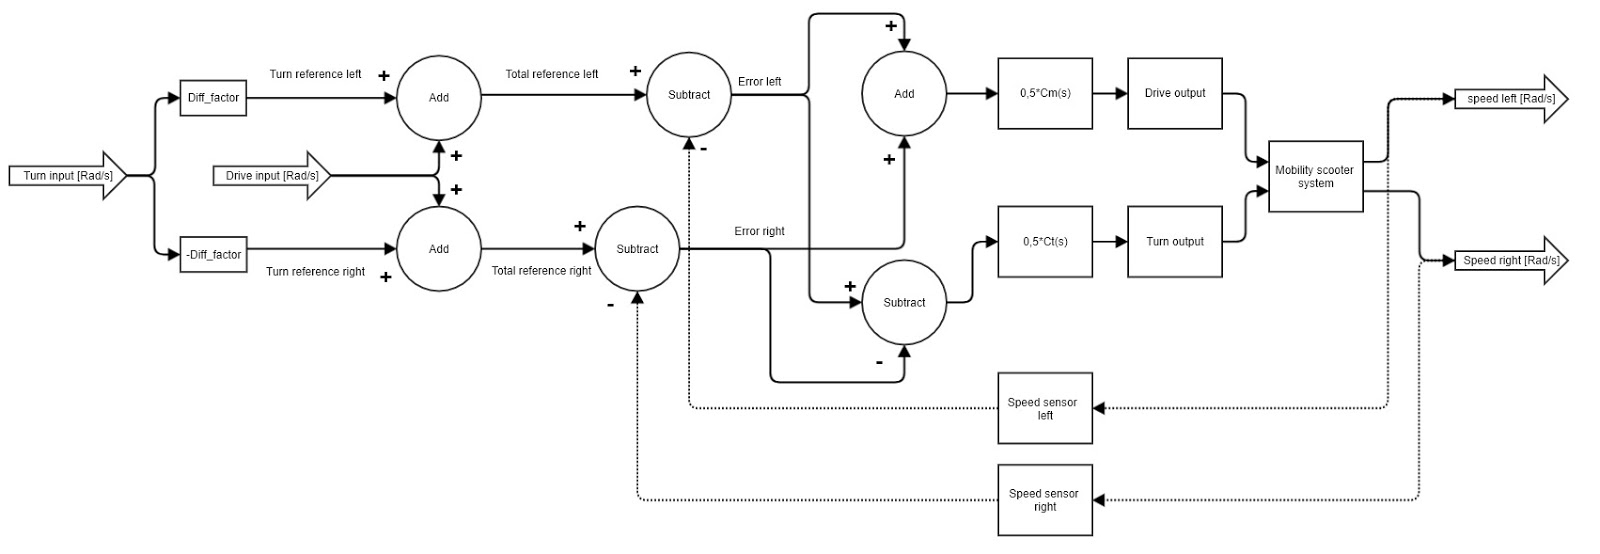
\includegraphics[width=15cm]{BlockDiagramCLCSR0.jpg}
\caption{Overview of the system integrated with closed loop control system}
\label{fig::controldiagram}
\end{figure}


\begin{figure}[H]
\begin{tabular}{|l|l|C{4cm}|C{4cm}|c|c|}
\hline
\textbf{Nr.} 		& \textbf{Variable(s)	}& \textbf{Left(+)}	&\textbf{Right(-)}							& \textbf{Min}	& \textbf{Max} 	\\ \hline
1		& Input Turn		& \multicolumn{2}{c|}{ Turn\_ Input}				& -		& -		\\ \hline
2		& Input Drive	& \multicolumn{2}{c|}{ Turn\_ Input}				& - 		& -		\\ \hline
3		& Reference Drive& \multicolumn{2}{c|}{ Drive\_ ref = Drive\_ Input}	& -		& - 		\\ \hline
4		& Reference Turn	&  $ Turn\_ Ref\_ L = Turn\_ Input * Diff\_ factor \footnote{difference in max speed of the wheel while turning compared to max speed while driving straight} $  & $ TUrn\_ Ref\_ R = -Turn\_ Input * Diff\_ Factor $ & - & - \\ \hline
5		& Total Reference Speed & $Tot\_ Ref = Drive\_ Ref + Turn\_ Ref\_ L$ & $Tot\_ Ref\_ R = Drive\_ Ref + Turn\_ Ref\_ R $ & -&- \\ \hline
6		& Measured\footnote{Sensors must be able to determine turning direction} & Speed\_ Sensor \_ L & Speed\_ Sensor\_ R & - & - \\ \hline
7		& Error & $Error\_ L = Tot\_ Ref\_ L - Speed\_ Sensor\_ L$ & $Error\_ R = Tot\_ Ref\_ R - Speed\_ Sensor \_ R$ & - & - \\ \hline
8		& Drive Output & \multicolumn{2}{c|}{$0.5 * (Error\_ L + Error\_ R) * C_m (S)$} & -100 & 100 \\ \hline
9		& Turn Output  & \multicolumn{2}{c|}{$0.5 * (Error\_ L - Error\_ R) * C_m (S)$} & -100 & 100 \\ \hline
\end{tabular}
\caption{Overview of input and outputs in the closed loop system}
\label{tab::closedoverview}
\end{figure}

\newpage

\section{Physical problems}
WTR's problems are not limited to its rear wheels.
The front wheels have their share of problems as well.

\subsection{Loose Batteries}
Generally speaking, when something goes wrong electrically, it is because a wire has come loose.
WTR has a different problem, which is illustrated in figure ~\ref{fig::batteries}.

\begin{figure}[H]
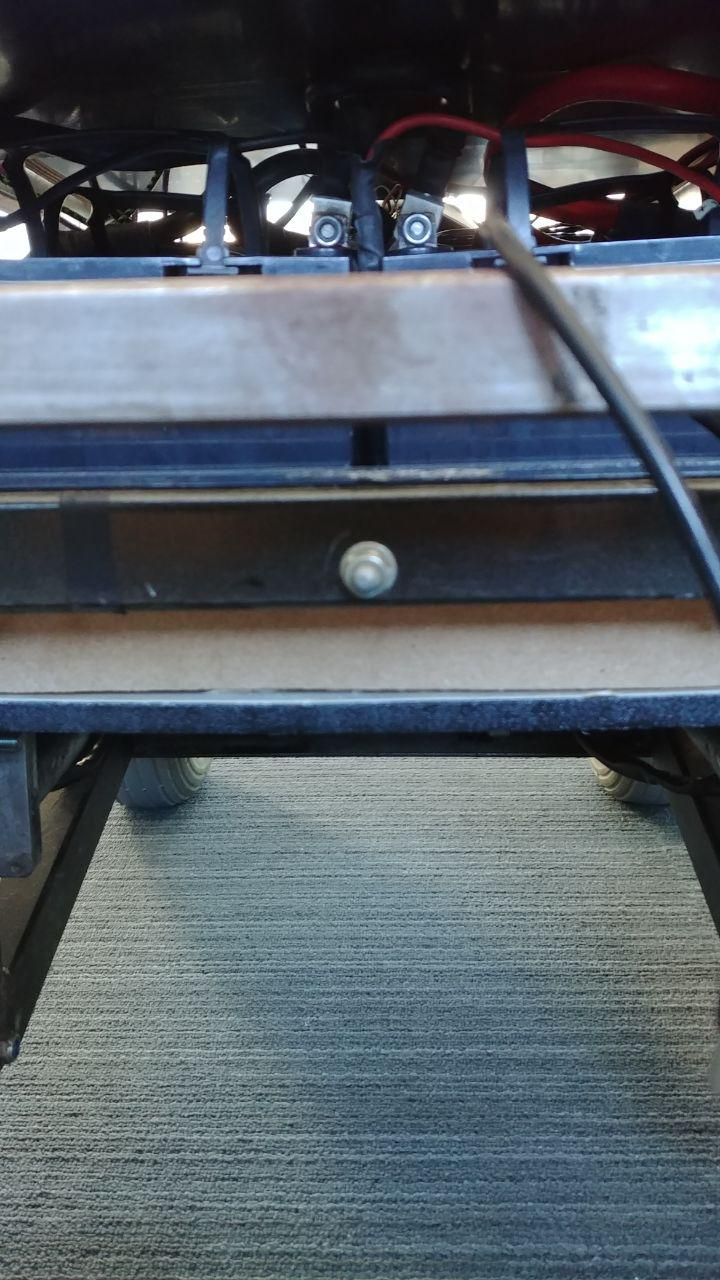
\includegraphics[width=8cm]{batteries.jpg}
\caption{As is slightly visible, the wooden plank is bending}
\label{fig::batteries}
\end{figure}

The wooden plank the batteries are resting on is bending, and the glue/tape which was used to attach that plank is letting go.
While the current situation is not immediately concerning, if WTR were to hit a bump and the force of all the batteries were to hit the plank at once it could snap off of break in two.
That would be a lot of clean-up and work for the group.

Another issue is that the batteries don't have a proper mount, so nothing really keeps them from sliding about.
This means a shifting weight within WTR, which is detrimental to the accuracy of its driving.

\subsubsection{solutions}
These issues are easy enough to resolve.
For the first issue, a metal L-joint around the center of the plank would reinforce the structure so that the bottom falling out would become much less likely.

The second issue can be resolved easily (though not very neatly) by simply wedging some wood or spare non-conductive material between the batteries to keep them from shifting around.
The neater but more time and effort consuming method would be to create a frame that goes over the batteries keeping them in place.


\subsection{After Effects of Collisions}
WTR is getting along in its age.
This is the 4th year of its life, and as such it has had to deal with a fair few knocks and scrapes.
One such collision ended up knocking one of the front wheels so that it was stuck at an angle.
As a result, the wheel kept scraping against the frame, and the effects can still be seen in figure ~\ref{fig::wheelclip}

\begin{figure}[H]
\centering
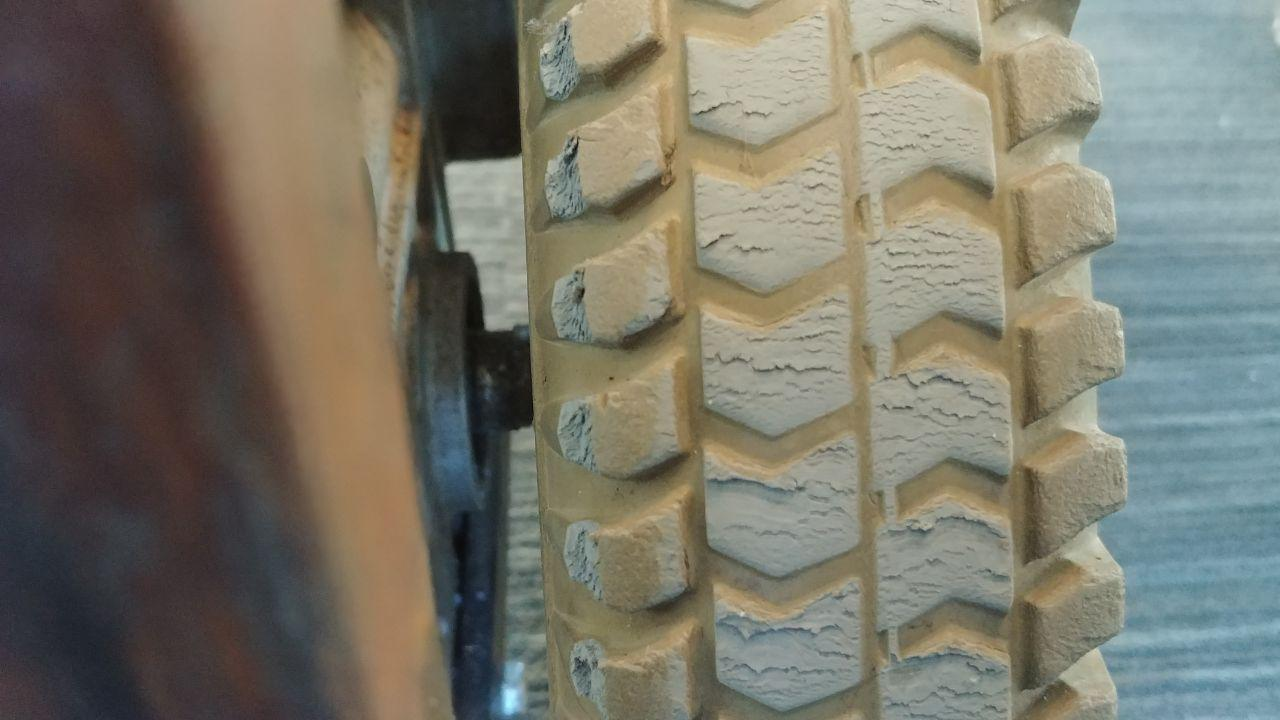
\includegraphics[width=12cm]{clippedwheel.jpg}
\label{fig::wheelclip}
\caption{The left side of the wheel shows the damage done by the frame.}
\end{figure}

Another issue which can be seen on figure ~\ref{fig::wheelclip} is that the tread on the tires is being worn away.
This results in the wheels slipping on the floors of Windesheim, which are mostly smooth, where they are not carpeted.
Since the two wheels are at different levels of wear due to the aforementioned grinding of the tire against the frame, they slip different amounts.
This unfortunately means that the accuracy of any soft-ware based solutions will be lessened.

\subsubsection{Solutions}
The effects mentioned above can be counteracted.
When it comes to the clipping issue on the left front tire, it has already been resolved by straightening out the axle and increasing the rigidity of the suspension, causing WTR to stand a little taller and putting a bit of distance between the tire and the frame.

The issue of slipping is not as easy to resolve.
New tires would be a lot of trouble to acquire and replace, and would at best be a stop-gap measure.
Because WTR is so heavy, even without the cover, the tires would get worn down quickly anyway.
The best solution therefore is to either lighten WTR, or attempt to reduce the impact of the slipping.

By adding rotary encoders, the amount of rotations made by both wheels can be tracked, so if one tire keeps slipping, the other can reduce its speed to compensate for the turn that would be caused by the different speeds of both sides of WTR.





\newpage
\appendix % all sections after this are appendices
\section{Glossary}
\begin{itemize}
\item \label{trm::dms} Dead-man's switch - a button on a controlling unit which has to be held down in order to have the robot respond to inputs. This is generally done in order ensure a machine cannot perform any actions should the controller be dropped or receive inputs without proper supervision.
\item WTR - Willy The Robot.
\end{itemize}
% Bibliography:
\newpage
\bibliographystyle{ieeetr}
\bibliography{references}


\end{document}
